\documentclass[11pt,a4paper]{article}
\usepackage{amsthm,amsmath,amsfonts,exscale,latexsym,graphicx}
\usepackage{times}
\usepackage{natbib}
\usepackage[usenames]{color}
\usepackage[pagebackref,colorlinks=true,breaklinks,linkcolor=Gray,citecolor=Gray,urlcolor=Gray,bookmarks,pdfpagemode=UseOutlines,pdftitle={Project Proposal: Round Trip Loss for Machine Translation}]{hyperref}

\bibliographystyle{apalike}
%shortcuts
\def\beq{\begin{equation}}
\def\eeq{\end{equation}}
\begin{document}
\title{Round Trip Loss for Machine Translation}
\date{\today}
\author{
Anja Adamov$\mbox{}^a$\thanks{\emph{E-mail address:} adamova@student.ethz.ch},
Lauro B\"{o}ni$\mbox{}^b$\thanks{\emph{E-mail address:} laboeni@gmail.com},
Simon A.\ Broda$\mbox{}^c\mbox{}^d$\thanks{\emph{E-mail address:} simon.broda@uzh.ch},
Urs V\"{o}geli$\mbox{}^b$\thanks{\emph{E-mail address:} voegeli.urs@gmail.com}
\medskip \\
\textit{\small $\mbox{}^a$IBM Switzerland Ltd., Zurich, Switzerland}
\medskip \\
\textit{\small $\mbox{}^b$ETH Zurich}
\medskip \\
\textit{\small $\mbox{}^c$Department of Banking and Finance, University of Zurich}
\medskip \\
\textit{\small $\mbox{}^d$Quantitative Economics Section, University of Amsterdam}
}
\maketitle \setcounter{page}{0}\thispagestyle{empty}
\definecolor{Gray}{rgb}{0.5,0.5,0.5}
\begin{abstract}
We augment a machine translation system with a round-trip loss to encourage the system to generate translations that, when translated back into the source language, retain much of the original structure. We surmised that in doing so, the model would learn internal representations with improved semantic meaning. Alas, this conjecture was not borne out by the results; our experiments show that incorporating the proposed loss has little to no effect on the obtained translations in terms of their BLEU scores.
\end{abstract}
\bigskip \textbf{Key Words}: Cycle consistency loss; deep learning; natural language understanding; machine translation; round-trip loss.
%\renewcommand{\baselinestretch}{1.3}\small\normalsize
\newpage
\setcounter{page}{1}
\section{Introduction}
Machine translation is an important task within the field of natural language understanding. Consequently, a variety of models have been proposed for solving it. One of the first truly successful models was the sequence-to-sequence (seq2seq) model of \citet{seq2seq}, while the current state of the art builds upon the \emph{Transformer} architecture introduced by \citet{transformer}. At a high level, both the seq2seq and the Transformer architectures are comprised of an encoder and decoder; the encoder learns an internal representation of the source sentence, and the decoder decodes it into the target language. For these models to work, the internal representation must capture the semantic meaning of the source sentence.

Irrespective of the architecture, these models are typically trained with the cross-entropy loss between the ground truth and predicted sentences, usually with teacher forcing.
Here, we propose to add a round-trip penalty to the loss function of the model. The idea is that instead of training a single model to translate from a source language $\mathcal{S}$ to a target language $\mathcal{T}$, one trains two models (of identical structure), one mapping $\mathcal{S}\mapsto \mathcal{T}$ and one mapping $\mathcal{T}\mapsto \mathcal{S}$. In this paper, we rely on the Transformer architecture of \citet{transformer}, but the idea applies to any encoder-decoder architecture.\footnote{We originally experimented with a seq2seq model, but found training to be too slow.} The two models are, at first, trained independently and in parallel, by feeding in the same batches of sentence pairs . After $\tau$ epochs, the models are then trained jointly, using as loss a sum of four cross-entropy terms, viz.,
\begin{equation}
\mathcal{L} = CE(s, \hat{s}) + CE(t, \hat{t}) + \lambda \left( CE(s, \tilde{s}) + CE(t, \tilde{t})\right).
\label{eq:RTL}
\end{equation}
Here, $s\in\mathcal{S}$ is the ground truth sentence in the first language, $t\in\mathcal{T}$ is the corresponding ground truth in the second language, $\hat{s}\in\mathcal{S}$ and $\hat{t}\in\mathcal{T}$ are the respective translations of $t$ and $s$, $\tilde{s}$ is obtained by translating $\hat{t}$ back to $\mathcal{S}$, and $\tilde{t}$ is obtained by translating $\hat{s}$ back to $\mathcal{T}$. $\tau$ and $\lambda$ are hyperparameters.

The round-trip loss is inspired by the cycle consistency loss pioneered by \citet{CycleGAN2017} in the context of GANs. The only application of this concept to the field of machine translation of which we are aware is \citet{su:2018}, who adapt it for unsupervised multi-modal machine translation. Here, we apply the idea to supervised machine translation, motivated by the intuition that encouraging the model to generate round-tripable translations may help it learn a semantically meaningful representation. A related idea is that of back-translation, pioneered by \citet{backtrans}. \citeauthor{backtrans} propose to augment the parallel training corpus used to train a machine translation system with synthetic data, obtained by translating a monolingual corpus in the target language to the source language using an independently trained system. They argue that this is beneficial in particular when parallel training data is scarce. The difference with our approach is two-fold: i) in our approach, the two networks are trained \emph{jointly}, each with their own round-trip loss term, whereas in back-translation, the models are trained separately, with only one of them benefiting from back-translation; ii) we do not assume the existence of a separate monolingual corpus in the target language, but work strictly with a parallel corpus. Having ground truth available, we are thus able to use teacher forcing in constructing the round-trip loss contribution, greatly speeding up training.

The remainder of this manuscript is organized as follows. Section \ref{sec:models} describes the model architecture and our implementation of it. Section \ref{sec:results} details the results of our experiments with the proposed round-trip loss. Section \ref{sec:discussion} provides a discussion and concludes.

\section{Models and Methods}\label{sec:models}
\subsection{Model Architecture}
%Unless explicitly stated otherwise, this section is based on \cite{transformer}. Useful background %information on Recurrent and Convolutional Neural Networks is based on \cite{Goodfellow-et-al-2016}.
For deep neural networks to perform sequence translation, some form of memory is required, as words in a sequence generally depend on words in other parts of the sequence. As an example, completing  the phrase ``My father is a winegrower, so unsurprisingly he likes to drink \ldots'' is greatly aided by the context provided earlier in the sequence.

Recurrent neural networks achieve this via an autoregressive structure. Their downside is that they are inherently sequential in nature, rendering them difficult to parallelize and hence computationally suboptimal.
Convolutional neural networks, on the other hand, are easily parallelizable, but mostly exploit local structure while struggling with long-term dependencies. 

\begin{figure}[ht]
    \centering
    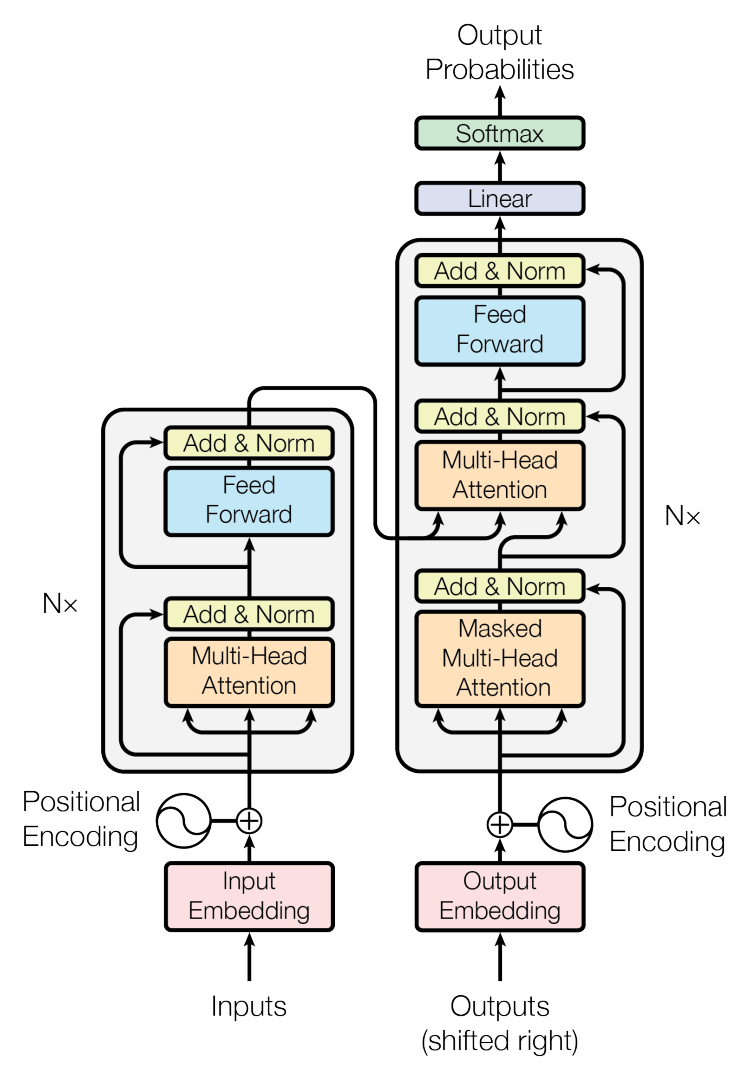
\includegraphics[scale=0.45]{images/Transformer.PNG}
    \caption{Architecture of the Transformer model. Image credit: \cite{transformer}.}
    \label{fig:transformer}
\end{figure}

The Transformer model solves this dilemma by exclusively relying on attention --- or more precisely, self-attention --- to capture global dependencies between input and output, without relying on recurrence or convolutions.
The model consists of an encoder and decoder, each of which stacks $N$ identical layers  (the base Transformer in \citet{transformer} uses $N=6$). The encoder maps the input sequence to a continuous representation, which is in turn used by the decoder to generate the output sequence.

The first encoder layer takes as input a positional encoding and the embeddings of the input sequence generated by an embedding layer. The positional information allows the Transformer to use the order of the sequence.

Each encoder layer consists of two components: a multi-headed self-attention layer and a feed-forward neural network, with residual connections around them. The self-attention mechanism takes an input vector of length $d_{\text{model}} = 512$ from the previous layer and projects it to obtain eight key, value, and query vectors of length $64$, one each for every attention head. An attention head uses the query and key vectors to generate a softmax over the values and computes its output by multiplying the values and the softmax activations. The outputs of all attention heads are then concatenated to a vector of length $d_{\text{model}}$ and fed through the feed-forward network, which consists of two linear layers, the inner of which has size $d_{\text{ff}} = 2048$). The outputs of the feed forward network are passed to the next encoder layer.


The decoder layers are similar, but add one more sublayer: a masked attention mechanism over the encoder outputs. The final decoder layer is followed by a linear layer and a softmax layer to produce the desired output probabilities. The model architecture is visualized in Figure \ref{fig:transformer}.

\subsection{Implementation and Training Details}
We use the Transformer implementation in TensorFlow 2.0 available from the \href{https://www.tensorflow.org/tutorials/text/transformer}{tensorflow website} and implement a custom training loop, which instantiates the $\mathcal{S}\mapsto\mathcal{T}$ and $\mathcal{T}\mapsto\mathcal{S}$ models and trains them jointly with the loss described in \eqref{eq:RTL}. Our code is available at \href{https://github.com/s-broda/nmt}{https://github.com/s-broda/nmt}. 

We train our models on the WMT'14 English -- German data set available from \linebreak\href{https://nlp.stanford.edu/projects/nmt/}{https://nlp.stanford.edu/projects/nmt/}. The training set consists of 4,508,785 sentence pairs, of which we retain those where source and target sequence both have a length of 40 or fewer tokens to keep the computational demands manageable (the original Transformer model in \citet{transformer} uses a maximal sequence length of 65). We employ a subword tokenizer and experiment with relatively small target vocabulary sizes ($2^{13}$ and $2^{14}$), again to keep computational demands at bay (a production system would likely use a vocabulary at least twice as large). Compared to the base Transformer, we also reduce the number of layers from 6 to 4, $d_{\text{model}}$ from 512 to 128, and $d_{\text{ff}}$ from 2048 to 512. The number of attention heads is kept at 8.
With these choices, training the model (which consists of two Transformers) for a single epoch on the entire dataset takes about 72 minutes on a single NVIDIA GTX1080 Ti. We use the same learning rate schedule as \cite{transformer}, which slowly increases the learning rate to around 0.0014 over 4000 warmup steps, and decays it thereafter.


At test time, we rely on the beam search decoder implementation from \href{https://github.com/tensorflow/tensor2tensor/blob/master/tensor2tensor/utils}{tensor2tensor}. We use a beam width of 10 and a length penalty of $\alpha=0.65$, per the recommendations of \citet{googlenmt}. We assess the quality of the translations of the 3,003 sentences in the test set using the BLEU score \citep{bleu}, computed using the \href{https://www.nltk.org/}{nltk} package. Only the translations from $\mathcal{S}$ (German) to $\mathcal{T}$ (English) are scored.




\section{Results}\label{sec:results}
%\subsection{Experiments}
In order to evaluate the effect of our proposed round-trip loss, we conduct a number of experiments. First, we train and evaluate the model from scratch for different values of $\lambda$.  This corresponds to setting $\tau=0$ in \eqref{eq:RTL}. We observe that validation accuracy stops improving after about 15 epochs, so this is the value we use throughout (unless noted otherwise). The results after training each model for these 15 epochs are shown in Table \ref{tab:result1}.

\begin{table} [ht]
\centering
\small
\begin{tabular}{ l || c | c | c | c | c | c | c | c | c  }
  $\lambda$ & 0.0 & 0.02 & 0.05 & 0.1 & 0.2 & 0.3 & 0.4 &  0.6 \\ \hline
  $\nu=2^{13}$ & 11.69 & 11.00 & 10.34 & \textbf{11.89} & 10.65 & 9.75 & 11.29 &  11.19 \\
  $\nu=2^{14}$ & \textbf{12.38} & 11.81 & 12.04 & 12.11 & 12.23 & 12.15 & 11.80 &  11.68 \\
\end{tabular}
\caption{BLEU scores for models trained from scratch, for different target vocabulary sizes $\nu$.}
\label{tab:result1}
\end{table}

The results are, at best, inconclusive. For vocabulary size $\nu=2^{13}$, while the best BLEU score is obtained with $\lambda=0.1$, there is very little variation in the resulting BLEU scores within the range of $\lambda$ values tested. With vocabulary size $\nu=2^{14}$, the picture is similar, although the best score is now obtained with $\lambda=0$ (i.e., no round trip loss). While we have not formally tested this, the variation in scores appears small enough to be entirely attributable to random fluctuations. 

In order to verify that the round-trip loss has any effect at all (and to rule out an error in our implementation), we trained a model with the unreasonably large value of $\lambda=100$. This resulted in a BLEU score of less than 0.1, confirming that the round-trip loss does eventually have an effect on the results, albeit a negative one in this case.

In our next set of experiments, we pre-train a model without round-trip loss ($\lambda=0$), and then fine-tune it for another 15 epochs using the same values for $\lambda$ as before. This corresponds to a non-zero value of $\tau$ in \eqref{eq:RTL}. As before, we use both $2^{13}$ and $2^{14}$ as our vocabulary size, and set $\tau=12$ for the former and $\tau=15$ for the latter. For comparison, we also trained a model with $\lambda=0$ for $\tau+15$ epochs. The results are shown in Table \ref{tab:result2}.

\begin{table} [ht]
\centering
\small
\begin{tabular}{ l || c | c | c | c | c | c | c | c | c  }
  $\lambda$ & 0.0 & 0.02 & 0.05 & 0.1 & 0.2 & 0.3 & 0.4 & 0.6 \\ \hline
  $\nu=2^{13}$ & \textbf{12.24} & 12.05 & 11.72 & 11.83 & 11.95 & 12.07 & 11.94 & 11.67 \\
  $\nu=2^{14}$ & \textbf{13.27} & 11.52 & 12.62 & 12.86 & 12.71 & 12.59 & 12.60 & 12.44 \\
\end{tabular}
\caption{BLEU scores for pre-trained models after fine tuning for 15 epochs, for different target vocabulary sizes $\nu$.}
\label{tab:result2}
\end{table}

The results are qualitatively similar to those without pre-training, except that the best score is now obtained with $\lambda=0$ for both vocabulary sizes. As before, what little difference exists between models appears attributable to random variation.

Finally, we conducted a last set of experiments in which we aimed to compare our proposed round-trip loss to the back-translation approach of \citet{backtrans}. Note that even when trained without round-trip loss ($\lambda=0$), our implementation always trains two models jointly, one for translating $\mathcal{S}\mapsto\mathcal{T}$ and one for $\mathcal{T}\mapsto\mathcal{S}$. Thus, after training on a subset of the data for 15 epochs, we used the model to translate part of the remaining training data from $\mathcal{T}\mapsto\mathcal{S}$, and then augmented the training data in the source language with these synthetic data. We then trained a model from scratch on this augmented data set and evaluated it as usual. Unfortunately, these experiments were heavily constrained by computational time, mostly because translation is very costly: our implementation will translate roughly 3,000 sentences per hour. As such, we decided to back-translate only around 0.5\% (21,600 sentences) of the training data. To allow this small augmentation to make a difference, we restricted the ground truth part of the data to 10\% of its original size. We also restrained ourselves to a tokenizer with a target vocabulary size of  $2^{13}$ to further reduce computational cost.\footnote{We experimented both with using the original tokenizer trained on the entire dataset, and a tokenizer trained on only the subset used for training.} With these restrictions, all models (with and without round trip loss)  resulted in BLEU scores below 1. These do not allow for a proper comparison and are thus not reported here.


%\subsection{Example Translations}

\section{Discussion and Conclusions}\label{sec:discussion}
In this work, we proposed to augment a neural machine translation system with a round-trip loss, inspired by the cycle consistency loss of \citet{CycleGAN2017}. In our experiments, we were unable to demonstrate any effect of the additional loss term, positive or negative, for a range of weights. We did, however, find that the additional loss term does have an effect when given extremely large weight. As such, it is conceivable that further experimentation with moderately large weights might find more encouraging results. 

These results notwithstanding, we maintain that some form of regularization towards round-tripable translations should be able to improve translation quality, both because of the strong intuitive appeal of the idea, and because of its relation to the rather successful concept of backtranslation. An alternative to the approach pursued herein would be to add a regularization term that penalizes the squared norm of the difference between the outputs of the encoders of the two models $\mathcal{S}\mapsto\mathcal{T}$ and $\mathcal{T}\mapsto\mathcal{S}$. We leave these experiments to subsequent work.
\newpage
\bibliography{proposal}
\end{document}

